\section{Analysis and Discussion}

\section{Analysis of Data}
The visualiser created in section \ref{vis} was used to analyse the trend in sentiment from different perspectives.

\subsection{Longitudinal analysis}\label{ana:long}
The Independent archive scraped contains articles from 2011 to 2018, offering just over seven years of news. When the headline and body's sentiment were initially analysed, there was a high noise level present in the data, as shown in appendix \ref{app:vis-ind-raw}. However, a rolling average was applied using the smoothing feature of the visualiser, and a more apparent trend appeared, shown in figure \ref{fig:smooth-ind}.

\begin{figure}[ht!]
  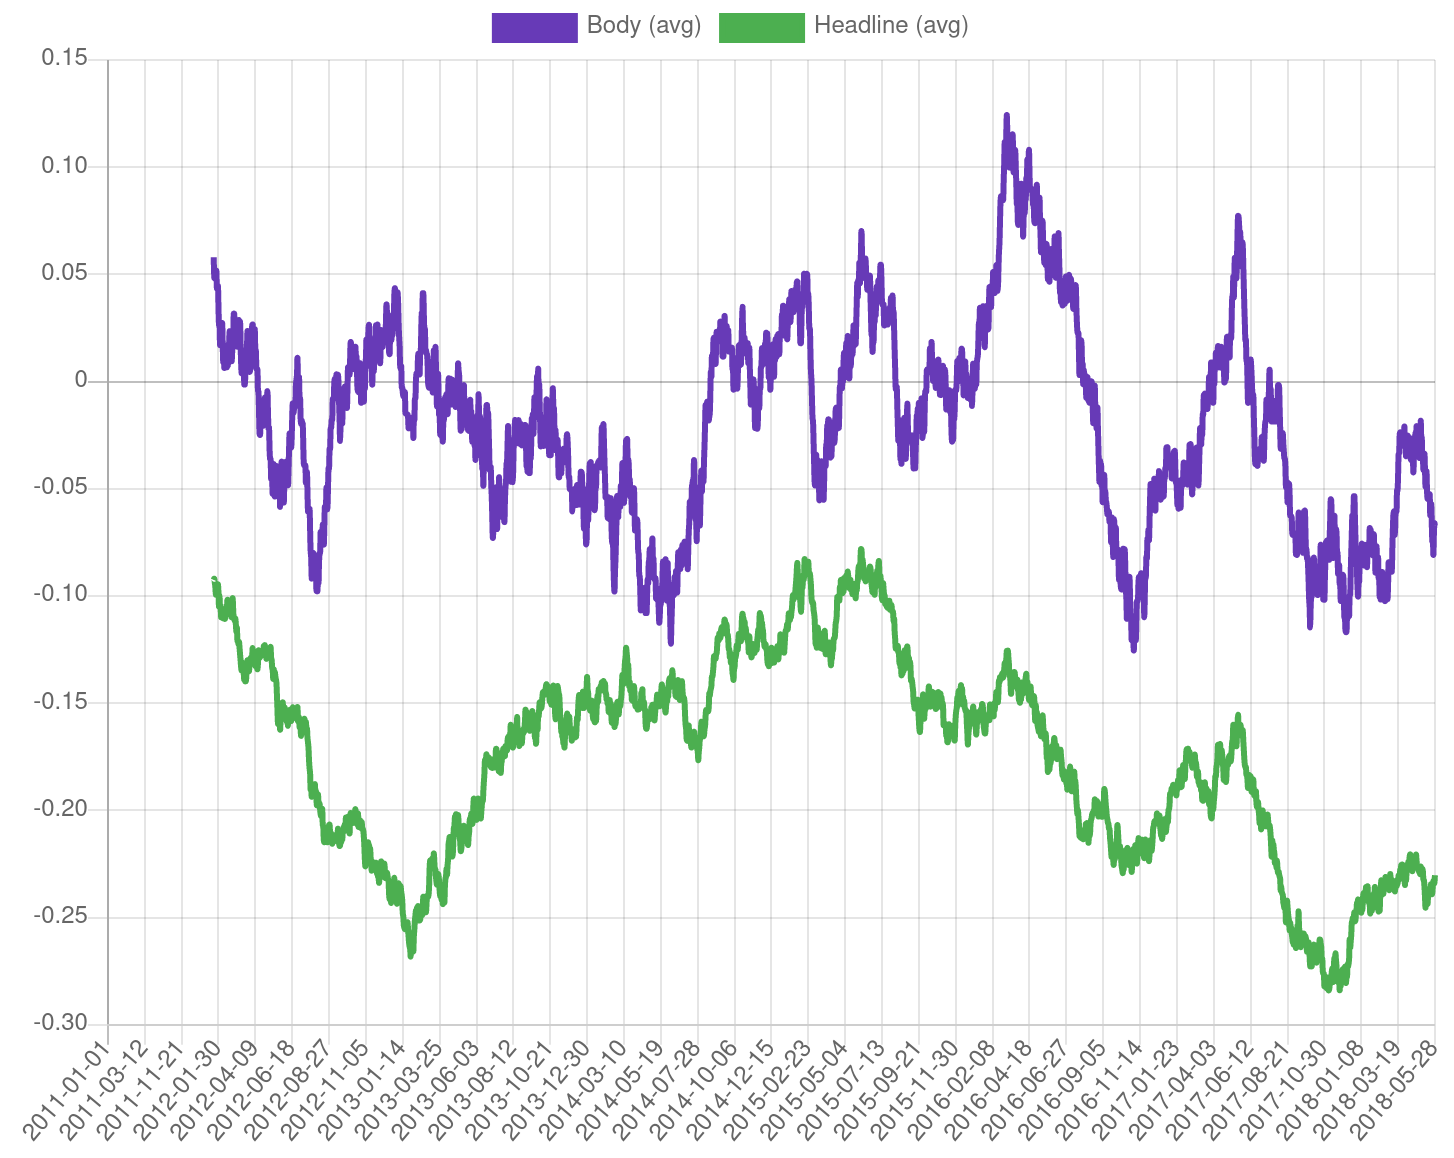
\includegraphics[width=\linewidth]{../visualisation/ind-smooth.png}
  \caption{A chart to show the difference between headline and body sentiment of the Independent archive.}
  \label{fig:smooth-ind}
\end{figure}

The first thing of note in the above chart is that the headline is, on average, consistently more negative than the body of a news article. This trend supports the study conducted by \citeA{arango2014}, who determined that bad news sells more magazines than good news. This finding means that a news story's negative aspects are more likely to be exaggerated and played up in the article's headline to increase revenue.

Although an average article's headline is has a more negative sentiment than the article's content, there is a direct relationship between the two - for instance, when the sentiment of the body peaks in June 2017, the headline's sentiment mirrors this with a peak of its own. An exception to this is the dip of headline sentiment in 2013, which is not reflected in the body's trend. 

The peaks and troughs in the data can also be linked to national and global events. The UK voted to leave the European Union on the 23rd of June 2016, followed by a period of political and economic instability. On the chart, a steep decline in the sentiment of articles bodies can be seen in June. As The Independent is a paper with a pro-market stance, it makes sense that their reporting's negativity mimics the strong downward trend of the FTSE. However, due to the rolling average in place, the data points cannot be tied down to a specific date, so any connection between the trends shown and real-life events is spurious.

\subsection{Cross sectional analysis}

Articles from a cross-section of news sources had been collected from a 3-month time period. As with the previous chart, when the headline sentiment of each of these sources was analysed, it produced a very incoherent and noisy output, as shown in appendix \ref{app:vis-all-raw}. However, some clear trends surfaced when a rolling average was applied, shown below in figure \ref{fig:smooth-all}. Note that while the visualiser was used to generate the raw data, the resultant graph was created using a separate script \footnote{\url{https://github.com/jacobbarrow/honours/blob/master/visualisation/comparison.py}}. This is because the visualiser has been designed to compare different analysis approaches instead of different data sources, so it is unable to plot different sources on the same chart.

\begin{figure}[h]
  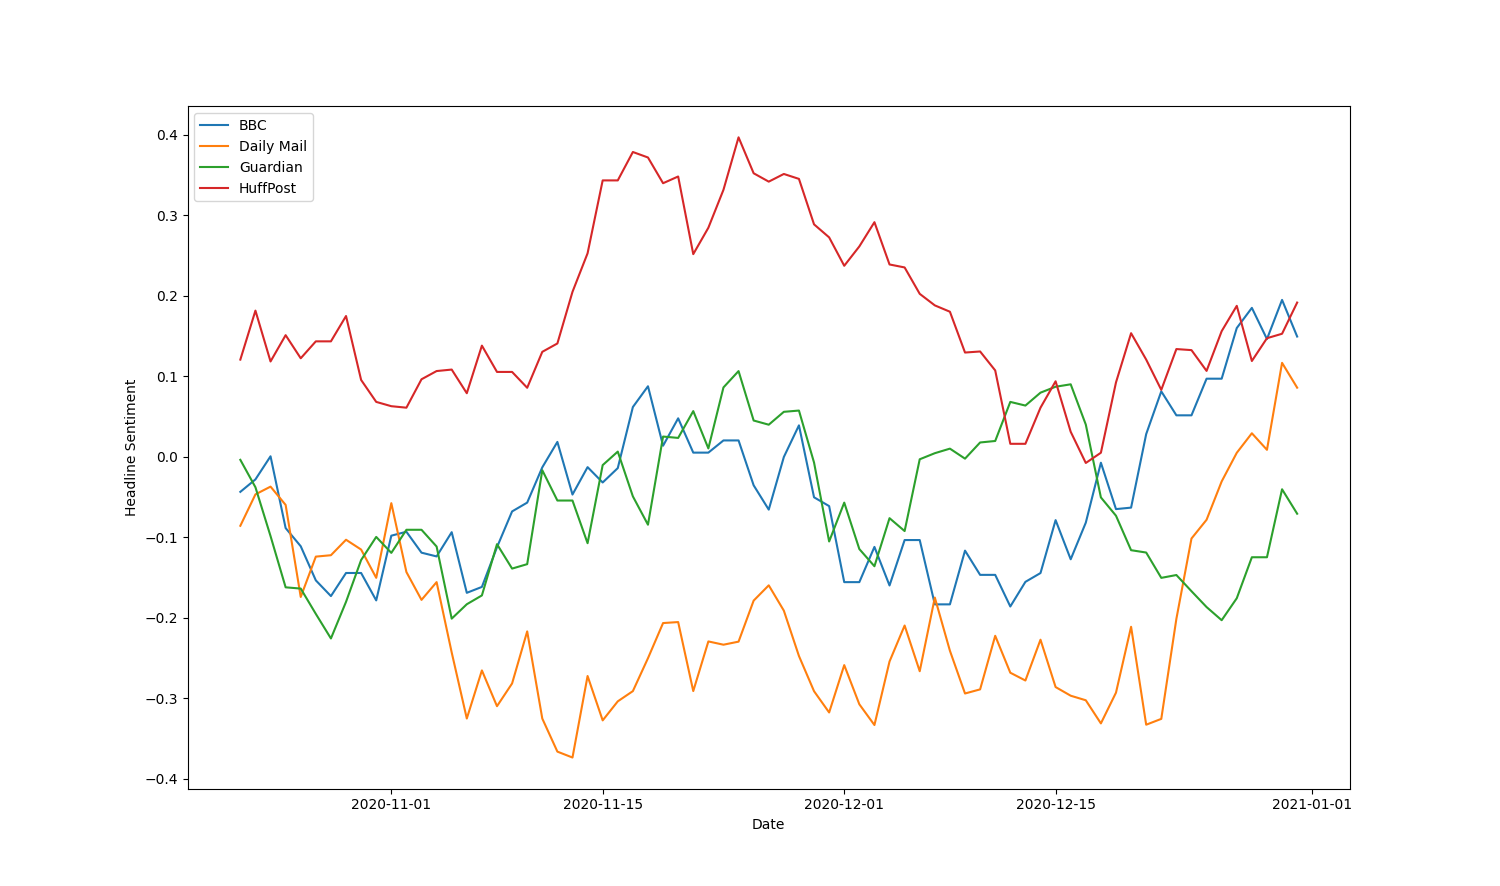
\includegraphics[width=\linewidth]{../visualisation/comparison-smooth.png}
  \caption{A chart to show the difference in headline sentiment between several news outlets}
  \label{fig:smooth-all}
\end{figure}

One of the trends that appears in the chart is that the Huffington Post has the most positive headlines, whereas the Daily Mail has the most negative headlines. A possible explanation for this is that the Daily Mail typically manufactures outrage, whereas the Huffington Post generally produces list-based articles and stories not generally linked to current affairs (e.g., 'Comic Relief: 7 Highlights From This Year's Red Nose Day Telethon'\footnote{\url{https://www.huffingtonpost.co.uk/entry/red-nose-day-2021-best-bits-funniest-highlights_uk_6055be48c5b6f12839d47dfe}} and 'The Bread Cutting Hack You Never Knew You Kneaded'\footnote{\url{https://www.huffingtonpost.co.uk/entry/bread-cutting-hack_uk_60547026c5b6d6c2a2a663b1}}). 

Another interesting trend is the peak in the average sentiment of all sources towards the end of the year. This could be because of the Christmas holidays, or even because the general sentiment at the time is that the new year would mark a change in the tide of the pandemic \footnote{\url{https://www.independent.co.uk/news/uk/home-news/covid-vaccine-climate-change-remote-working-b1768098.html}}\footnote{\url{https://www.aarp.org/health/conditions-treatments/info-2020/coronavirus-2021.html}}.

\section{Conclusion}

From the experiments conducted in section \ref{experimentation} and the review of the literature in section \ref{lit}, it is clear the statistical natural language processing methods are not sufficient to identify the nuances of incongruence. 

While classical approaches can identify the general gist of a piece of text, articles can become incongruent through a subtle remark or a seeming off-hand turn of phrase, which cannot be detected using the methods investigated in this project. 

\subsection{Analysis against the project aims}

In section \ref{int:qs}, several research questions are posed that this project sought to answer.

The second question has been addressed in section \ref{ana:long} - the language of news articles has varied considerably over the past decade and followed trends that closely mirror real-world events.

The third question has been considered throughout this dissertation - statistical NLP cannot determine the congruence of a news article's headline using the approaches investigated here. This ties closely with the first question, which has gone unanswered. As a classifier was not created, analysis on the collected dataset can not be undertaken. It is hoped a future researcher will seek to answer this unresolved question.

\subsection{Analysis against the work of others}

As mentioned at the end of the literature review (section \ref{lit:sum}), statistical NLP has not been applied to incongruence detection before, making a comparison against other's work difficult.

However, others have also found limitations of statistical NLP. \citeauthor{manning1999} finds that problems arise when classical NLP techniques are given to long, complicated sections of text - the approaches used are unable to produce 'grammatical judgements' for convoluted sentences. This mirrors the difficulties faced in this project - while a headline's meaning is relatively simple to extract, understanding a long news article and distilling it to a single 'truth' is where the challenge lies.

\citeauthor{sag2002} also ran into problems with NLP. They found that multi-word expressions (such as 'every which way'), particularly idioms (such as 'kick the bucket'), tend to cause issues for NLP. This is because they may subvert a grammatical rule and could require cultural context to have meaning. In the setting of this project, a similar issue arises. News article headlines often use idioms and short, catchy phrases to draw in a reader with humour. For instance, in the (fictional) headline 'Heinz CEO spills the beans in this exclusive interview', the idiom 'spills the beans' is used to construct a pun, with great effect. However, this headline may be misinterpreted by a congruence classifier; seeing no mention of a bean spillage, it could incorrectly mark the article's headline as incongruent.

\subsection{Self Apprasial}

This section provides a review from a personal perspective, and as such uses an informal writing style.

I have found myself challenged in several aspects of this project and encountered several difficulties. I had previously not explored NLP and found a great deal of time covering the foundations and gaining a broad understanding. However, I found this very enjoyable and felt more confident in my abilities by the end of the literature review.

Additionally, the lack of similar work in the field posed an issue. There was no clear starting point and no guarantee that I would produce a positive result. This was, at times, frustrating, and at certain points I found myself needing further motivation and guidance, for which I am thankful to my supervisor.  While the inability to produce a classifier is disheartening it raises a series of interesting questions, listed above. With hindsight, I would have researched more NLP approaches to be able to produce a broader set of experiments.

Aside from these challenges, the project has gone smoothly. I was able to manage my time well, writing considerable chunks of the dissertation in tandem with developing the code required. I made sure to start the data collection process as soon as I could, as it was clear from the outset it would take several months. 

My well-planned project management left me with plenty of excess towards the end of the project. I used this to both add some polish to the literature review and to also work on some additional features, such as the data visualisation website.

Overall, while some issues and setbacks have occurred, they have been well managed, and the majority of the project has progressed well, gradually building a knowledge base, collecting a dataset and running a series of experiments.


\subsection{Future Work}

While this project has failed to create a classifier capable of detecting incongruent news headlines, in every other respect, it has been a success; the groundwork has been laid for future research and development in many forms. 

Firstly, several approaches have been considered and discounted through empirical testing, and a framework for experimentation has been proposed. This will save future researchers the time and effort of starting from scratch and provide a baseline standard against which to compare their results. It has been suggested that a machine learning approach, utilising a neural network, could be an appropriate next step.

Although a substantial labelled data source was not created, the framework for labelling and a website to allow individuals to rate articles has been implemented. With either a wide network of willing volunteers or a small amount of funding, a large labelled dataset can be created, which can then be used to train a classifier or act as a gold standard of truth.

Additionally, a visualiser has been created. This proof-of-concept website has been made with future development in mind, and while only one form of experiment has been implemented (sentiment analysis), it can be easily extended. This will allow future researchers to analyse their results without having to create a bespoke graphing platform. 

Finally, a vast dataset of 345k articles has been produced spanning several decades and from various sources. Included within these articles is a snapshot of the UK media as it reported on the most deadly pandemic to impact the nation since influenza in 1919. This wealth of data will hold a plethora of trends and insights waiting to be uncovered.

Some broad questions have arisen from this work and could be used as prompts for further study:
\begin{itemize}
	\item Why is statistical NLP insufficient to detect incongruence in text?
	\item To what extent are the articles in the collected dataset congruent?
	\item What other trends in the dataset can be unearthed?	
\end{itemize} 

\subsection{Final Thoughts}

Throughout this project, it has become clear that statistical natural language techniques are not capable of detecting the twists and turns that news editors employ, intentionally or not, to mislead and deceive their readers. There is just too much nuance involved, and subtle misdirection is at play that conceals the true meaning of an article. This is a non-trivial problem that, if solvable, will require a great deal of research and computational power to overcome.

Nonetheless, the project has explored the breadth of NLP, as well as looking at classical techniques in depth. It has produced a range of outputs, from tools to help others collect and visualise data to a substantial set of articles that span over half a century of national news. It is hoped that this work will be continued, and future researchers uncover more trends and produce a classifier capable of detecting incongruent articles.

